% !TEX root =  main.tex

% Chapter of 2-5 pages about torque ctrl, robust inv dyn and mujoco, 
% Use a high-level viewpoint, stressing the challenges of the proposed approach, almost no equation (similar to CR research project)
\section{Controlling the Motion on the Robot}
Once we have computed a trajectory of the CoM associated with a discrete sequence of contact configurations, we need to address the problem of how to execute this motion on a physical robot.
Clearly, different ways exist to tackle this problem.
Here we present the approach that we believe to be the best, and then we discuss the associated challenges and issues.

The main challenge when working on a real robot is the presence of uncertainties.
In the absence of uncertainties, planned motions could be directly executed on the robot.
Uncertainties make the robot deviate from the planned trajectories in unpredictable ways.
Our goal here is to react to these deviations (i.e. tracking errors) so as to get the robot to the desired final configuration without falling.

The specific features of legged robots make this task extremely hard.
First, these systems are subject to many constraints: motor torque and velocity bounds, joint position bounds, contact force friction cones, (self-)collisions.
This is clearly problematic because tracking errors may lead to constraint violations, which are typically connected to failure and damages of robot and/or environment.
Second, their dynamics is unstable and discontinuous (making/breaking contacts introduces discontinuities).
This means that small variations in control inputs or initial state may result in large variations of the future state.

\subsection{Model Predictive Control}
We believe that the best tool to control a constrained and unstable dynamical system is Model Predictive Control (MPC).
MPC consists in solving a discrete-time finite-horizon optimal control problem (OCP) and then using only the first part of the resulting control trajectory.
The process is repeated as fast as possible using the latest state estimation as initial state.
MPC has been successfully used for the control of chemical processes.
However, applications on legged robots are much more challenging:
\begin{itemize}
\item \textbf{High dimensionality}: solving an optimization problem is computationally demanding, especially when the size of state and control are large (around 60 for humanoids)
\item \textbf{Discontinuities}: the optimization process is slowed down by the discontinuities in the system dynamics, which need either to be approximated through smoothing~\citep{Todorov} or to be handled through hybrid models~\citep{Diehl2009a}.
\item \textbf{Non convexity}: the optimal control problem is not convex, so it needs to be properly initialized to converge to a \emph{``good-enough''} local minimum.
\end{itemize}
These challenges make it impossible to solve a new OCP at each sensor reading (typically every 1 ms) as we would like to. 
In practice we may only be able to do it every 10-100 sensor readings---which for a full humanoid still requires an extremely efficient implementation. 
In between two MPC computations we can still use the last-computed open-loop control trajectory.
In 2015 we reported the first application of whole-body nonlinear MPC on a humanoid robot (i.e. HRP-2)~\citep{Koenemann2015}.
\begin{figure}[!tbp]
\begin{center}
	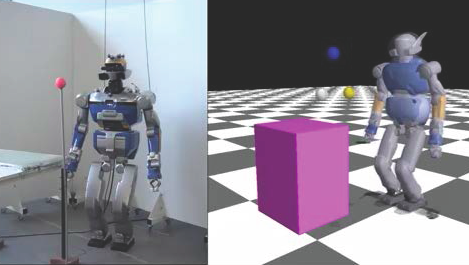
\includegraphics[width=0.4\textwidth]{figures/mujoco/ss0.png} \quad
	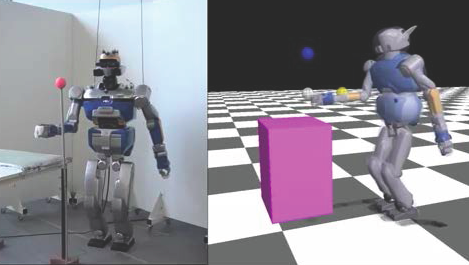
\includegraphics[width=0.4\textwidth]{figures/mujoco/ss1.png} \\
	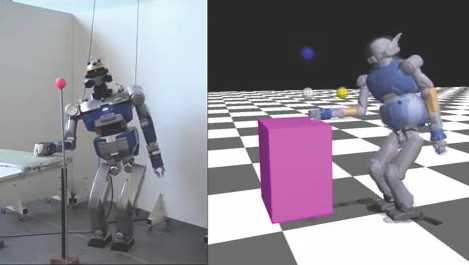
\includegraphics[width=0.4\textwidth]{figures/mujoco/ss2.png} \quad
	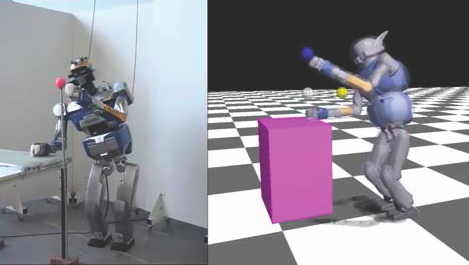
\includegraphics[width=0.4\textwidth]{figures/mujoco/ss3.png}
	\caption{Whole-body multi-contact experiment on HRP-2. The robot reaches for a target while it uses a table as an additional support to keep balance.}
	\label{fig:mujoco}
\end{center}
\end{figure}
To do that we used the efficient optimal-control framework MuJoCo~\citep{Todorov}, which can compute a 500ms trajectory for a 25-DoF robot in 50ms on a standard desktop computer.
Fig.~\ref{fig:mujoco} shows one of the experiments: HRP-2 reaches for a target making contact with a table for support.


\subsection{Constraint Robustness}
MPC inherently provides some level of robustness to uncertainties thanks to the frequent updates of the control trajectory based on the sensor feedback.
However, nothing prevents the solver to compute state-control trajectories that are close to the margins of their feasible sets.
When this happens, there is a high probability of violating some constraints, which often results in failure.
To solve this issue we can account for uncertainties in the OCP formulation, which leads us to \emph{Robust MPC}~\citep{Bemporad1999}.
While Robust MPC is an interesting and promising control paradigm, to the best of our knowledge it has never been used on legged robots.
The main reason is probably the computation time: in general Robust MPC is more computationally demanding than standard MPC, whose computation time is already the bottleneck for application on legged robots.

Despite this unpromising premise, the robotics community has recently started to study and apply robust control~\citep{Brasseur2015, Nguyen} and planning algorithms~\citep{Luo, Mordatch2015}.
In particular, we recently proposed an optimization-based inverse-dynamics control framework that tries to guarantee constraint satisfaction despite errors in the joint-torque tracking~\citep{DelPrete2015b}.
The accuracy of the torque tracking is known to be an important issue~\citep{Boaventura2012b, DelPrete2015a} (as we discuss at length in the next section), in particular for robots that do not have access to a direct measurement of the joint torques---such as most current humanoid robots: HRP-2, Hubo, Atlas, Valkyrie, Asimo, iCub. 
\begin{figure}[htbp]
   \centering
   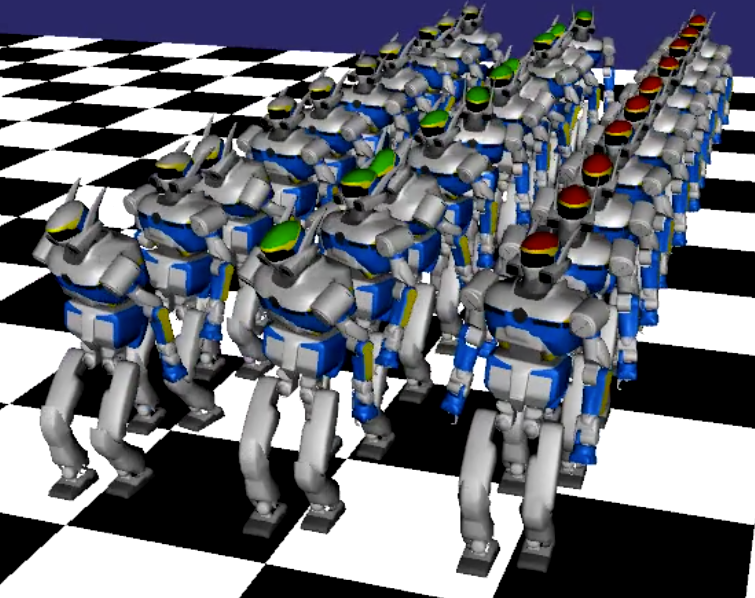
\includegraphics[width=0.5\textwidth]{figures/30_robots_walking.png} % requires the graphicx package
   \caption{Simulation of 30 HRP-2 robots walking in the presence of uncertainties, the goal being to compare the classic controller (left line) to the proposed robust controllers: stochastic (central line) and worst-case (right line).}
   \label{fig:robust_TSID}
\end{figure}
We validated the proposed methods on a simulated HRP-2 humanoid robot performing walking (see Fig. 1) and manipulation tasks, for which we presented statistics based on several batches of 100 tests each; in each batch we simulated different uncertainties.
We empirically showed that taking robustness into account greatly increases the chances of the robot not to fall, even in the presence of other uncertainties: velocity-estimation delays, inertial-parameter inaccuracies and limited actuator bandwidth. 
Moreover, we verified that we could solve the proposed optimization problems in less than 1 ms on a standard CPU, so that these formulations are suitable for online control.

Even if inverse-dynamics control is know to be more prone to myopic behaviors than MPC, these results encourage us to move forward towards Robust MPC.
However, the step from robust inverse dynamics to Robust MPC is not trivial and several concerns need to be addressed.
\begin{itemize}
\item Will the (likely) increased computation time be outweighed by the improved robustness?
\item Should we adopt an open-loop or a close-loop prediction scheme? In the presence of uncertainties, the classic open-loop prediction scheme used in MPC results in a pessimistic prediction of the future, which does not account for the fact that only the first value of the control trajectory is applied, and then the optimization is repeated using the new measurement. Open-loop prediction results then in too conservative behaviors, and close-loop prediction should be preferred. However, the latter results in an intractable optimization, which needs to be approximated---e.g. by assuming a linear feedback control law for the prediction.
\item Should we optimize performance for the nominal model or worst-case scenario? Considering the worst-case scenario leads to a minimax optimization that is in general much harder to solve; moreover, it can result in a too conservative behavior of the system.
\end{itemize}


\subsection{Joint Torque Control}
Another issue that we need to address for the real-robot implementation is the control of the actuators.
Typically whole-body control and planning assume joint torques as the control inputs.
However, real actuators are far from being the perfect torque source that we would like them to be.
This is due to the large friction in the transmission mechanisms (e.g. gear boxes, pistons).
Currently, the best solution seems to use joint-torque feedback~\citep{Albu-Schaffer2007, Boaventura2012b}.
Since in general this controller is not computationally demanding, it is better to decouple it from the whole-body MPC so as to run it at higher frequency (i.e. 1-3 kHz).

Despite being an essential component for the implementation of inverse-dynamics control, the problem of regulating the joint torques is still subject of ongoing research. The difference between the various works mainly lies in the type of actuator (rigid vs elastic, electric vs hydraulic) and the chosen actuator model (i.e. whether it includes the gear-box elasticity and/or the electric motor pole).

Our approach was to neglect the elasticity of the harmonic drive and the electric pole of the motor transfer function, which results in an instantaneous relationship between motor input and joint torque. 
While the model has experimentally proved to achieve a reasonable accuracy, it remarkably simplifies the identification procedure: in particular, we do not need to excite the robot at high frequencies. 
Most torque controllers rely on a direct measure of the joint torques. 
Since our robot is not equipped with joint-torque sensors, we estimate the joint torques using the procedure proposed for iCub~[4]: we propagate the wrenches measured by the F/T sensors (located at ankles and wrists) along the kinematic chain using a model of the dynamics of the robot and an estimation of velocities and accelerations of the robot bodies, reconstructed using the joint encoders and the IMU. 
This joint-torque estimation is used in the control to servo a feedback; it is also used offline to identify the relationship between the motor input and the associated joint torque. 
The torque-control law is a simple superposition of a feedforward term (given by the identified motor model) and a feedback term (based on the estimated joint torque). 
We validated the whole framework by implementing an inverse-dynamics controller on one leg of HRP-2, which has 6 joints. 
In comparison to the closed-source position control of HRP-2, we get a better position tracking while using lower feedback gains (up to 25\%). 
We also show the performances of our framework on a force-tracking task, which is easily integrated in the inverse-dynamics controller.
